\begin{figure}[h]
    \centering
    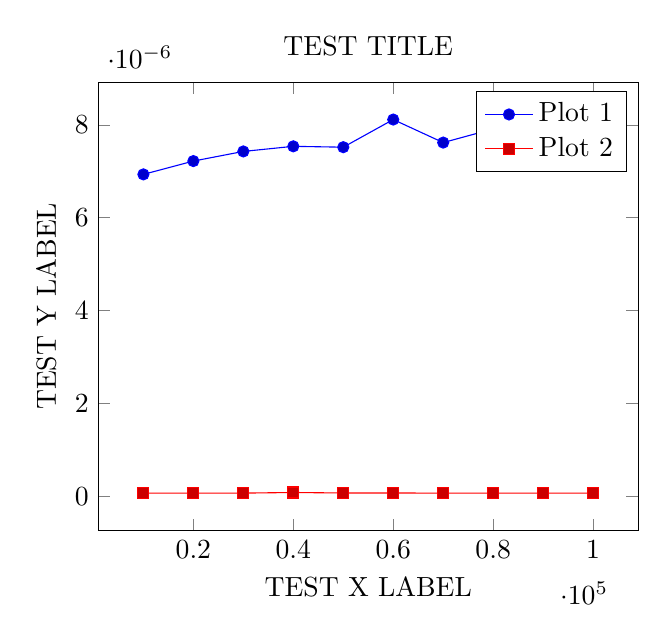
\begin{tikzpicture}
        \begin{axis}[
            xlabel={TEST X LABEL},
            ylabel={TEST Y LABEL},
            title={TEST TITLE}
        ]
		\addplot coordinates {
			(10000, 6.933658602697013e-06)
			(20000, 7.219775172611076e-06)
			(30000, 7.427586154969745e-06)
			(40000, 7.537515152884033e-06)
			(50000, 7.5188422820053894e-06)
			(60000, 8.11396474742665e-06)
			(70000, 7.618230143133564e-06)
			(80000, 7.911574921129593e-06)
			(90000, 7.978737021225424e-06)
			(100000, 7.994096963399588e-06)
		};
		\addplot coordinates {
			(10000, 7.167973014698959e-08)
			(20000, 7.167973014698959e-08)
			(30000, 7.198090548321545e-08)
			(40000, 8.523262030069035e-08)
			(50000, 7.408913284079333e-08)
			(60000, 7.439030817746329e-08)
			(70000, 7.137855480987553e-08)
			(80000, 7.137855481031963e-08)
			(90000, 7.137855480987553e-08)
			(100000, 7.107737947364967e-08)
		};
        \legend{Plot 1, Plot 2}
        \end{axis}
    \end{tikzpicture}
    \caption{TEST CAPTION}
\end{figure}